\section*{Ex.~2.1 (15 pts) --- Schedule diagrams: Round-Robin, FIFO and SJF}

Task set $(a_i, e_i)$: $T_1(1,10)$, $T_2(2,4)$, $T_3(3,1)$, $T_4(4,6)$.

\paragraph{Conventions.}
\begin{itemize}\itemsep0pt
  \item Time is discrete: the task dispatched at instant $t$ holds the CPU over $[t,t+1)$, and a task with arrival time $a_i$ is runnable at instant $a_i$.
  \item Nothing has arrived before $t=1$, so $[0,1)$ is idle under every policy; it is drawn, not cropped.
  \item FIFO is non-preemptive and dispatches in arrival order.
  \item SJF is the classical non-preemptive form: at each dispatch point it picks the arrived, unfinished task with the smallest \emph{total} execution time, and that task then runs to completion.
  \item Round-Robin uses $q=1$. Where a task arrives at the same instant that the running task exhausts its quantum, the arriving task is enqueued first and the preempted task then joins the tail of the ready queue.
  \item Every tie --- equal bursts in SJF, equal standing in the ready queue --- goes to the smaller index.
\end{itemize}

Total busy time is $10+4+1+6=21$ units, so with the single idle unit all three policies complete at $t=22$.

\begin{figure}[H]
  \centering
  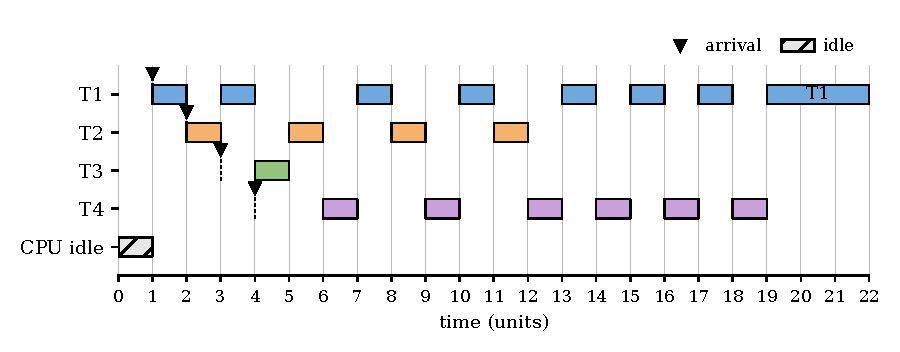
\includegraphics[width=\linewidth]{fig_p1_rr.pdf}
  \caption{Round-Robin, $q=1$.}
  \label{p1:fig:rr}
\end{figure}

\begin{figure}[H]
  \centering
  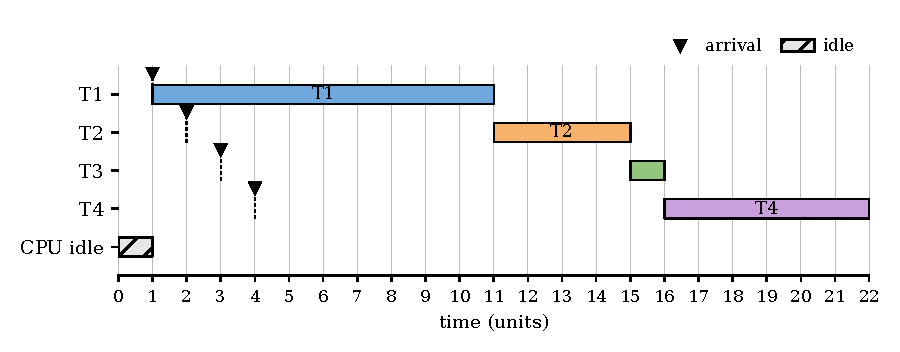
\includegraphics[width=\linewidth]{fig_p1_fifo.pdf}
  \caption{FIFO (non-preemptive).}
  \label{p1:fig:fifo}
\end{figure}

\begin{figure}[H]
  \centering
  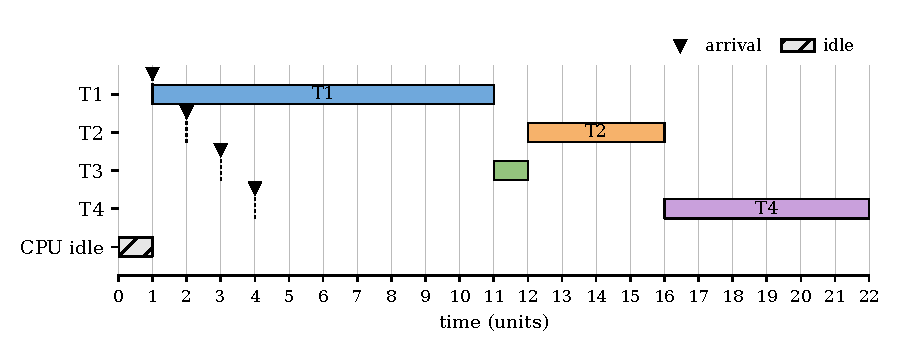
\includegraphics[width=\linewidth]{fig_p1_sjf.pdf}
  \caption{SJF (non-preemptive).}
  \label{p1:fig:sjf}
\end{figure}

\begin{table}[H]
  \centering\footnotesize
  \begin{tabular}{@{}lcc*{9}{c}@{}}
    \toprule
    & & & \multicolumn{3}{c}{Round-Robin ($q=1$)} & \multicolumn{3}{c}{FIFO} & \multicolumn{3}{c}{SJF} \\
    \cmidrule(lr){4-6}\cmidrule(lr){7-9}\cmidrule(lr){10-12}
    Task & $a_i$ & $e_i$ & $C$ & $T$ & $W$ & $C$ & $T$ & $W$ & $C$ & $T$ & $W$ \\
    \midrule
    $T_1$ & 1 & 10 & 22 & 21 & 11 & 11 & 10 & 0  & 11 & 10 & 0  \\
    $T_2$ & 2 & 4  & 12 & 10 & 6  & 15 & 13 & 9  & 16 & 14 & 10 \\
    $T_3$ & 3 & 1  & 5  & 2  & 1  & 16 & 13 & 12 & 12 & 9  & 8  \\
    $T_4$ & 4 & 6  & 19 & 15 & 9  & 22 & 18 & 12 & 22 & 18 & 12 \\
    \midrule
    \multicolumn{3}{@{}l}{average} & & 12.00 & 6.75 & & 13.50 & 8.25 & & 12.75 & 7.50 \\
    \bottomrule
  \end{tabular}
  \caption{Completion $C$, turnaround $T=C-a_i$ and waiting $W=T-e_i$ times.}
  \label{p1:tab:times}
\end{table}

Round-Robin gives the lowest average turnaround and waiting times because the three short
tasks interleave with $T_1$ instead of queueing behind its 10-unit burst, and FIFO the
highest because $T_3$ waits 12 units to run for 1. The preemptive variant of SJF (SRTF)
would give a different schedule: $T_2$ preempts $T_1$ at $t=2$ and $T_3$ preempts $T_2$ at
$t=3$.
